%%%%%%%%%%%%%%%%%%%%%%%%%%%%%%%%%%%%%%%%%%%%%%%%%%%%%%%%%%%%%%%%%%%%%
% In English:
%    This is a Latex template for São Paulo Research Foudation (FAPESP)
%         reports (annual or final).
%    This is the modified version of the original Latex template from
%         following website.
%    Original Source: http://www.howtotex.com
%    For information about FAPESP, check http://www.fapesp.br/en
%    This template targets mainly on reports in Portuguese language.
%    New additions and changes in the latest version:
%        - Added the possibility of including multiple members in the
%          research team, with the commands \memberA{Name of Member A}
%          \memberB{Name of Member B} \memberC{Name of Member C} etc.
%        - Included commands to define project modality and the research
%          agency (if you want to use the same model for other research
%          agencies such as CAPES, CNPq etc).
%
% In Portuguese:
%    Este é um modelo Latex para relatórios (anual ou final) da Fundação
%         de Amparo à pesquisa do Estado de São Paulo (FAPESP).
%    Esta é uma versão modificada do modelo Latex do site supra mencionado.
%    Para informações sobre a FAPESP, verifique http://www.fapesp.br
%    Esse modelo foca principalmente nos relatórios escritos em Português.
%    Novas adições e alterações na última versão:
%       - Foi adicionada a possibilidade de incluir vários membros no
%         grupo de pesquisas, com os comandos \membroA{Nome do Membro A}
%         \membroB{} \membroC{} etc.
%       - Foram incluídos comandos para definir modalidade de projeto e
%         agência de fomento (caso queira utilizar o mesmo modelo para
%         outras agências, CAPES, CNPq etc).
%
% Author/Autor: André Leon Sampaio Gradvohl, Dr.
% Email:        andre.gradvohl@gmail.com
% Lattes CV:    http://lattes.cnpq.br/9343261628675642
% GitHub: http://gradvohl.github.io/
%
% Last update/Última versão: 19/Feb/2018
%
%%%%%%%%%%%%%%%%%%%%%%%%%%%%%%%%%%%%%%%%%%%%%%%%%%%%%%%%%%%%%%%%%%%%%%
\documentclass[12pt]{report}
\usepackage[a4paper]{geometry}
\usepackage[utf8]{inputenc}
\usepackage[english]{babel}
\usepackage[myheadings]{fullpage}
\usepackage[T1]{fontenc}
\usepackage{fancyhdr}
\usepackage{setspace}
\usepackage{sectsty}
\usepackage{url}

%%% iniciar capitulo na mesma pagina (Mateus) %%%
\usepackage{etoolbox}
\makeatletter %inicio da modificacao (iniciar capitulo na msma pag)
\patchcmd{\chapter}{\if@openright\cleardoublepage\else\clearpage\fi}{}{}{}
\makeatother %fim da modificacao
%%% iniciar capitulo na mesma pagina (Mateus) %%%

%%------
%% Comandos gerais
%% Observação: o arquivo "comandos.tex" tem que estar presente.
%%------
%%%%%%%%%%%%%%%%%%%%%%%%%%%%%%%%%%%%%%%%%%%%%%%%%%%%%%%%%%%%%%%%%%%%%
% In English:
%    This is a list of commands specification for FAPESP reports.
%
% In Portuguese:
%    Esta é uma lista de especificação de comandos para relatórios
% da Fundação de Amparo à pesquisa do Estado de São Paulo (FAPESP).
%
% Author/Autor: André Leon Sampaio Gradvohl, Dr.
% Email:        andre.gradvohl@gmail.com
% Lattes CV:    http://lattes.cnpq.br/9343261628675642
%
% Last update/Última versão: 11/Sep/2016
%%%%%%%%%%%%%%%%%%%%%%%%%%%%%%%%%%%%%%%%%%%%%%%%%%%%%%%%%%%%%%%%%%%%%%

\newcommand{\HRule}[1]{\rule{\linewidth}{#1}}
\setcounter{tocdepth}{3}
\setcounter{secnumdepth}{3}

\newcommand{\titulo}[1]{\def\meuTitulo{#1}}
\newcommand{\tituloIngles}[1]{\def\meuTituloIngles{#1}}
\newcommand{\numProjeto}[1]{\def\numFAP{#1}}
\newcommand{\tipoRelatorio}[1]{\def\tipoRelat{#1 }} %o espaço depois do #1 é importante
\newcommand{\modalidadeProjeto}[1]{\def\modProjeto{#1}}
\newcommand{\agFomento}[2]{\def\agFom{#1} \def\siglaAgFom{#2}} %extenso Sigla
\newcommand{\autor}[1]{\def\nomeAutor{#1}}
\newcommand{\cidade}[1]{\def\nomeCidade{#1}}
\newcommand{\universidade}[1]{\def\nomeUniversidade{#1}}
\newcommand{\faculdade}[1]{\def\nomeFaculdade{#1}}
\newcommand{\periodoVigencia}[1]{\def\periodVig{#1}}
\newcommand{\periodoRelatorio}[1]{\def\periodRelat{#1}}
\newcommand{\orientador}[1]{\def\nomeOrientador{#1}}

\newcommand\namegroup[3]{%
   \begin{minipage}[t]{0.4\textwidth}
   \hspace{0.6cm}
   \begin{tikzpicture}
   \node[anchor=south east,inner sep = 0](signF){\includegraphics[width=#3]{#2}};
   \end{tikzpicture}
   \vspace*{0.1cm}  % leave some space above the horizontal line
   \hrule
   \vspace{1mm} % just a bit more whitespace below the line
   \centering
   \begin{tabular}[t]{c}
   #1
   \end{tabular}
   \end{minipage}}

\author{}
\date{}

%Definição de membros da equipe de pesquisas
\newcommand{\membroA}[1]{\def\nomeMembroA{#1}}
\newcommand{\membroB}[1]{\def\nomeMembroB{#1}}
\newcommand{\membroC}[1]{\def\nomeMembroC{#1}}
\newcommand{\membroD}[1]{\def\nomeMembroD{#1}}
\newcommand{\membroE}[1]{\def\nomeMembroE{#1}}
\newcommand{\membroF}[1]{\def\nomeMembroF{#1}}

\newcommand{\Figure}[1]{Figura~\ref{fig:#1}}
\newcommand{\Table}[1] {Tabela~\ref{#1}}
\newcommand{\Equation}[1] {Equa\c{c}\~ao~\ref{#1}}
\newcommand{\addFigure}[3] { %Parametros scale, fig_name, caption
    \begin{figure}[!hbt]
      \centering
      \includegraphics[scale=#1]{figures/}
      \caption{#3}\label{fig:#2}
    \end{figure}
}

\newcommand{\geraTitulo}{
\clearpage
\begin{titlepage}
  \begin{center}
      \vspace*{-3cm}
       { \setstretch{.5}
         \textsc{\nomeUniversidade} \\
         \HRule{.2pt}\\
         \textsc{\nomeFaculdade}
       }

       \vspace{5.5cm}

       \Large \textbf{\textsc{\meuTitulo}}
 	  \HRule{1.5pt} \\ [0.5cm]
       \linespread{1}
       \large Final report on the activities
       %\ifdefined\tipoRelat
       %     \tipoRelat
       %\fi
       of the
       \ifdefined\modProjeto
           \modProjeto
       \fi
       ~project supported by the \agFom. \\
   	   \HRule{1.5pt} \\ [0.5cm]

       \ifdefined\numFAP
          Grant \texttt{\#\numFAP}, \siglaAgFom
          \\ [0.5cm]
       \fi
        Author: \nomeAutor \\
        Advisor: \nomeOrientador \\[5.cm]

        % aqui começa a adicao das linhas de assinatura
        %Aluno: \tikz\draw [thick,solid] (0,0) -- (6,0); \\[.5cm]
        %Orientador: \tikz\draw [thick,solid] (0,0) -- (5.5,0);


        %% Assinatura assinatura ASSINATURA
        %\namegroup{Researcher}{example-image-a}
        \namegroup{Researcher}{fig/assinatura-mateus.png}{5cm}
        \hspace{1.5cm}
        \namegroup{Advisor}{fig/placeholder.png}{1cm}

        %\begin{minipage}[t]{0.4\textwidth}
        %\vspace*{1.5cm}
        %\hrule
        %\vspace{1mm}
        %\centering
        %\begin{tabular}[t]{c}
        %Aluno
        %\end{tabular}
        %\hspace{1.5cm}
        %\begin{minipage}[t]{0.4\textwidth}
        %\vspace*{1.5cm}
        %\hrule
        %\vspace{1mm}
        %\centering
        %\begin{tabular}[t]{c}
        %Aluno
        %\end{tabular}
        %\end{minipage}
        %%\hfill

        \vfill

        {\normalsize  \nomeCidade, \today}
 \end{center}
 \end{titlepage}
}

\usepackage{titlesec}
\titleformat{\chapter}{\normalfont\LARGE\bfseries}{\thechapter}{1em}{}
\titlespacing*{\chapter}{0pt}{3.5ex plus 1ex minus .2ex}{2.3ex plus .2ex}

%----------------------------------------------------------------------
% Cabeçalho e rodapé
%----------------------------------------------------------------------
\pagestyle{fancy}
\fancyhf{} % Limpa todos os campos de header and footer fields
\renewcommand{\headrulewidth}{0pt}
\fancyfoot[R]{\thepage}

\addto\captions{\renewcommand{\contentsname}{Summary}}
\addto\captions{\renewcommand{\bibname}{Bibliography}}

%------
% Resumo e Abstract
%------
%%\newcommand{\Resumo}[1]{
%%   \begin{otherlanguage}{portuguese}
%%       \addcontentsline{toc}{chapter}{Resumo}
%%       \begin{abstract} \thispagestyle{plain} \setcounter{page}{2}
%%          #1
%%        \end{abstract}
%%   \end{otherlanguage}
%%} %end \Resumo

\newcommand{\Abstract}[1]{
   \begin{otherlanguage}{english}
      \addcontentsline{toc}{chapter}{Abstract}
      \begin{abstract} \thispagestyle{plain} \setcounter{page}{3}
       #1
      \end{abstract}
    \end{otherlanguage}
} %end \abstract

%------
% Folha de rosto
%------


\newcommand{\folhaDeRosto}{
   \chapter*{Project}
   \addcontentsline{toc}{chapter}{General Project Information}
   \begin{itemize}
      \item Title:
            \begin{itemize}\item[] \textbf{\meuTitulo} \end{itemize}
      \item Advisor:
            \begin{itemize}\item[]\textbf{Prof. \nomeOrientador}\end{itemize}
      \item Project host institution:
            \begin{itemize}
               \item[]\textbf{\nomeFaculdade \ da \nomeUniversidade}
            \end{itemize}
      \item Research team:
            \begin{itemize}
               \ifdefined\nomeMembroA
                 \item[]\textbf{\nomeMembroA}
               \else
                 \item[]\textbf{\nomeAutor}
               \fi
               \ifx\nomeMembroB\undefined\else \item[]\textbf{\nomeMembroB}\fi
               \ifx\nomeMembroC\undefined\else \item[]\textbf{\nomeMembroC}\fi
               \ifx\nomeMembroD\undefined\else \item[]\textbf{\nomeMembroD}\fi
               \ifx\nomeMembroE\undefined\else \item[]\textbf{\nomeMembroE}\fi
               \ifx\nomeMembroF\undefined\else \item[]\textbf{\nomeMembroF}\fi
             \end{itemize}

          \ifdefined \numFAP
             \item Research project number:
             \begin{itemize}
                 \item[]\textbf{\numFAP}
             \end{itemize}
          \fi
       \item Validity period:
            \begin{itemize}
               \item[]\textbf{\periodVig}
            \end{itemize}
       \item Period covered by this scientific report:
            \begin{itemize}
               \item[]\textbf{\periodRelat}
            \end{itemize}
   \end{itemize}
   \clearpage
}


%\newcommand{\folhaDeRosto}{
%   \chapter*{Informações Gerais do Projeto}
%   \addcontentsline{toc}{chapter}{Informações Gerais do Projeto}
%   \begin{itemize}
%      \item Título do projeto:
%            \begin{itemize}\item[] \textbf{\meuTitulo} \end{itemize}
%      \item Nome do pesquisador responsável:
%            \begin{itemize}\item[]\textbf{Prof. \nomeOrientador}\end{itemize}
%      \item Instituição sede do projeto:
%            \begin{itemize}
%               \item[]\textbf{\nomeFaculdade \ da \nomeUniversidade}
%            \end{itemize}
%      \item Equipe de pesquisa:
%            \begin{itemize}
%               \ifdefined\nomeMembroA
%                 \item[]\textbf{\nomeMembroA}
%               \else
%                 \item[]\textbf{\nomeAutor}
%               \fi
%               \ifx\nomeMembroB\undefined\else \item[]\textbf{\nomeMembroB}\fi
%               \ifx\nomeMembroC\undefined\else \item[]\textbf{\nomeMembroC}\fi
%               \ifx\nomeMembroD\undefined\else \item[]\textbf{\nomeMembroD}\fi
%               \ifx\nomeMembroE\undefined\else \item[]\textbf{\nomeMembroE}\fi
%               \ifx\nomeMembroF\undefined\else \item[]\textbf{\nomeMembroF}\fi
%             \end{itemize}
%
%          \ifdefined \numFAP
%             \item Número do projeto de pesquisa:
%             \begin{itemize}
%                 \item[]\textbf{\numFAP}
%             \end{itemize}
%          \fi
%       \item Período de vigência:
%            \begin{itemize}
%               \item[]\textbf{\periodVig}
%            \end{itemize}
%       \item Período coberto por este relatório científico:
%            \begin{itemize}
%               \item[]\textbf{\periodRelat}
%            \end{itemize}
%   \end{itemize}
%   \clearpage
%}

\usepackage[brazilian]{babel}
\usepackage[left=2.5cm,right=2.5cm,top=3cm,bottom=2.5cm]{geometry}
\usepackage{mathtools}
\usepackage{amsthm}
\usepackage{amsmath}
%\usepackage{nccmath}
\usepackage{amssymb}
\usepackage{amsfonts}
\usepackage{physics}
%\usepackage{dsfont}
%\usepackage{mathrsfs}

\usepackage{titling}
\usepackage{indentfirst}

\usepackage{bm}
\usepackage[dvipsnames]{xcolor}
\usepackage{cancel}

\usepackage{xurl}
\usepackage[colorlinks=true]{hyperref}

\usepackage{float}
\usepackage{graphicx}
%\usepackage{tikz}
\usepackage{caption}
\usepackage{subcaption}

%%%%%%%%%%%%%%%%%%%%%%%%%%%%%%%%%%%%%%%%%%%%%%%%%%%

\newcommand{\eps}{\epsilon}
\newcommand{\vphi}{\varphi}
\newcommand{\cte}{\text{cte}}

\newcommand{\N}{\mathbb{N}}
\newcommand{\Z}{\mathbb{Z}}
\newcommand{\Q}{\mathbb{Q}}
\newcommand{\R}{\vb{R}}
\newcommand{\C}{\mathbb{C}}
\renewcommand{\S}{\hat{S}}
%\renewcommand{\H}{\s{H}}

\renewcommand{\a}{\vb{a}}
\newcommand{\nn}{\hat{n}}
\renewcommand{\d}{\dagger}
\newcommand{\up}{\uparrow}
\newcommand{\down}{\downarrow}

\newcommand{\0}{\vb{0}}
%\newcommand{\1}{\mathds{1}}
\newcommand{\E}{\vb{E}}
\newcommand{\B}{\vb{B}}
\renewcommand{\v}{\vb{v}}
\renewcommand{\r}{\vb{r}}
\renewcommand{\k}{\vb{k}}
\newcommand{\p}{\vb{p}}
\newcommand{\q}{\vb{q}}
\newcommand{\F}{\vb{F}}

\newcommand{\s}{\sigma}
%\newcommand{\prodint}[2]{\left\langle #1 , #2 \right\rangle}
\newcommand{\cc}[1]{\overline{#1}}
\newcommand{\Eval}[3]{\eval{\left( #1 \right)}_{#2}^{#3}}

\newcommand{\unit}[1]{\; \mathrm{#1}}

\newcommand{\n}{\medskip}
\newcommand{\e}{\quad \mathrm{e} \quad}
\newcommand{\ou}{\quad \mathrm{ou} \quad}
\newcommand{\virg}{\, , \;}
\newcommand{\ptodo}{\forall \,}
\renewcommand{\implies}{\; \Rightarrow \;}
%\newcommand{\eqname}[1]{\tag*{#1}} % Tag equation with name

\setlength{\droptitle}{-7em}

\theoremstyle{plain}
\newtheorem{theorem}{Teorema}[section]
%\newtheorem{defi}[theorem]{Definição}
\newtheorem{lemma}[theorem]{Lema}
%\newtheorem{corol}[theorem]{Corolário}
%\newtheorem{prop}[theorem]{Proposição}
%\newtheorem{example}{Exemplo}
%
%\newtheorem{inneraxiom}{Axioma}
%\newenvironment{axioma}[1]
%  {\renewcommand\theinneraxiom{#1}\inneraxiom}
%  {\endinneraxiom}
%
%\newtheorem{innerpostulado}{Postulado}
%\newenvironment{postulado}[1]
%  {\renewcommand\theinnerpostulado{#1}\innerpostulado}
%  {\endinnerpostulado}
%
%\newtheorem{innerexercise}{Exercício}
%\newenvironment{exercise}[1]
%  {\renewcommand\theinnerexercise{#1}\innerexercise}
%  {\endinnerexercise}
%
%\newtheorem{innerthm}{Teorema}
%\newenvironment{teorema}[1]
%  {\renewcommand\theinnerthm{#1}\innerthm}
%  {\endinnerthm}
%
\newtheorem{innerlema}{Lema}
\newenvironment{lema}[1]
  {\renewcommand\theinnerlema{#1}\innerlema}
  {\endinnerlema}
%
%\theoremstyle{remark}
%\newtheorem*{hint}{Dica}
%\newtheorem*{notation}{Notação}
%\newtheorem*{obs}{Observação}

%
%%-----
%% Página de título
%% Observação: As definições que aparecem a seguir comporão a
%%             página de título e a folha de rosto.
%%-----
%% Define o nome da universidade onde o projeto foi desenvolvido.
\universidade{Universidade de São Paulo (USP)}
%
%% Define o nome da faculdade onde o projeto foi desenvolvido.
\faculdade{Instituto de Física}
%
%% Define o título do projeto.
\titulo{Multi-orbital topological Anderson models for twisted bilayer graphene}
%
%% Define a agencia de Fomento e a abreviatura. O primeiro argumento é o
%% nome por extenso e o segundo a abreviatura.
%% Ambos os argumentos são obrigatórios
\agFomento{São Paulo Research Foundation}{FAPESP}
%
%% Define o tipo de relatório. Pode ser Anual ou Final.
%% Não é obrigatório definir o tipo de relatório.
%\tipoRelatorio{Final}
%
%% Define a modalidade de Projeto. Pode ser temático, regular, etc.
\modalidadeProjeto{Master's degree}
%
%% Define o número do projeto.
%% Não é obrigatório definir o número do projeto.
\numProjeto{2023/02913-5}
%
%% Define o autor do relatório.
\autor{Mateus Marques}
\orientador{Dr. Luis Gregório G. V. Dias da Silva}
%
%% Define a equipe do projeto (incluindo o pesquisador responsável no comando \membroA{}
\membroA{Mateus Marques}
%% Inclua os demais membros do grupo (máximo +5)
\membroB{Luis Gregório G. V. Dias da Silva}
%\membroC{Francisco}
%\membroD{Joao}
%\membroE{Antonio}
%\membroF{José}
%
%% Define o período da vigência do Projeto.
\periodoVigencia{January 1, 2023 to December 31, 2024}
%
%% Define o período coberto pelo relatório.
\periodoRelatorio{January 1, 2023 to \today}
%
%% Define a cidade onde o projeto foi desenvolvido.
\cidade{São Paulo}

\newcommand{\ALERT}[1]{\textcolor{red}{#1}}

%%-----
%% Página de título
%% Observação: Os comandos a seguir não devem ser mudados,
%%             exceto caso necessário.
%%-----
\begin{document}
%
%% Define a numeração em romanos.
\pagenumbering{roman}
%
%% Gera a folha de título.
\geraTitulo
%
%% Gera a folha de rosto.
\folhaDeRosto
%
%% Escreva aqui o resumo em português. Fica no Resumo do Projeto Proposto
%\Resumo{
%Neste projeto estamos interessado apenas no valor da bolsa. Não fizemos praticamente
%nada nesse tempo e não pretendemos fazer. Eu apenas pretendo entregar este relatório
%para ficar tudo certo.
%}
%
%% Escreva aqui o resumo em inglês. NAO PRECISA
%\Abstract{
%Same thing but in english.
%}
%
%% Adicionará o sumário.
%% Mantenha o \thispagestyle{empty} e \clearpage
\tableofcontents
\thispagestyle{empty}
\clearpage
%
%% Define a numeração em arábicos.
\pagenumbering{arabic}

%%-----
%% Formatação do título da seção
%%-----
\sectionfont{\scshape}

%%-----
%% Corpo do texto
%%-----


%%-----
%% Resumo do projeto
%%-----
\chapter{Summary} \label{chp:abstract}

The twisted bilayer graphene (TBG) is a fascinating system that displays a plethora of intriguing physical phenomena such as correlated insulators, superconductivity \cite{cao2018}, and unconventional quantum Hall effects \cite{unconv_QHE_tbg_2006}, among others. Several recent experiments have demonstrated the rich electronic properties of TBG, which exhibits correlated insulating and superconducting phases. In spite of such a vast amount of experimental data, there are still several open questions regarding the theoretical description of this material in different regimes. While there is some consensus that these phenomena are related to the formation of flat bands near the Fermi level captured by non-interacting band structure models \cite{macdonald2011}, the description of TBG as a strongly correlated system is nonetheless challenging. In this Master's project, we propose a description of the correlated electronic properties of Magic-Angle TBG (MATBG) in terms of multi-orbital topological Anderson models (both as a single impurity and as a periodic Anderson lattice), building on the framework recently developed describing MATBG as a topological heavy fermion problem \cite{topoheavyfermion2022}. By employing a combination of analytical and numerical methods, we aim to study the low-energy physics of such models and identify the emergent energy scales and the nature of the Mott transition.

We plan to address the MATBG by initially studying a single impurity site localized at the origin using an impurity solver method. Our primary choice is the Non-Crossing Approximation (NCA) solver due to its low computational cost and capability to explore temperature effects \cite{impurity-solvers}. Following this, we aim to extend our approach to a periodic multi-orbital Anderson model by implementing the Dynamical Mean-Field Theory (DMFT) algorithm \cite{georges1996}, which involves iteratively calling the impurity solver at each step.

To establish a robust initial implementation of the impurity solver and DMFT, we begin our studies with the Hubbard model \cite{hubbard1963} on a Bethe lattice at the coordination number limit $z\to\infty$. This choice is motivated by the model's relative simplicity and its suitability as a benchmark for our DMFT code. In Section \ref{sec:hubbard}, we address the technical details of applying DMFT to this benchmark system and show our numerical results, which demonstrate the Metal-Insulator phase transition in both the particle-hole symmetric (PHS) case ($\epsilon_d = U/2$) and the asymmetric case.

In Section \ref{sec:tbg}, we present our progress in understanding the MATBG system by studying its geometry \cite{handbook2019}, the Bistritzer-MacDonald (BM) model \cite{macdonald2011}, and the Wannier obstruction phenomenon \cite{zou}. The Wannier obstruction, arising from the non-trivial topology, refers to the impossibility of representing the flat bands using exponentially localized Wannier functions that preserve all symmetries of the band structure.

\pagebreak


\chapter{Accomplishments in the period} \label{chp:accomplishments}

Throughout the period outlined in this report, our advancements comprised three primary activities: acquainting ourselves with the theory of Condensed Matter Physics, delving into numerical techniques (such as NCA and DMFT), and thoroughly reviewing the literature pertaining to the MATBG system of interest.

\begin{itemize}
\item The student completed four courses: Solid State I and II, Statistical Mechanics, and Group Theory Applied to Molecules and Solids. Each course was vital for understanding the general theory of many-body systems and for beginning the study of the MATBG system in question. In particular, the Group Theory course was crucial for comprehending the symmetry and topology aspects of MATBG. Additionally, the Hubbard model was extensively studied in Solid State II.

\item While our initial intention was to utilize the Hubbard model only for benchmarking DMFT, our endeavor led us to a comprehensive exploration of the Mott transition within this system, yielding original findings. In Section \ref{sec:hubbard}, we describe the techniques and concepts intrinsic to the DMFT framework, presenting our results on the Metal-Insulator transition. Additionally, the student enrolled in the supplementary course titled "Strong coupling theories for metal-insulator transitions: DMFT and beyond" at USP during the first semester of 2023. This course proved invaluable, offering insights into extending DMFT to complex systems.

\item We initiated our exploration of the MATBG theory with reference to \cite{handbook2019}, aiming primarily to comprehend the Moiré pattern geometry and the Bistritzer-MacDonald continuous model \cite{macdonald2011}. Subsequently, our focus shifted to analyzing the system's symmetries \cite{thesis_rennella}, which are pivotal, with implications such as the Wannier obstruction \cite{zou}. In Section \ref{sec:tbg}, we elucidate our studies.
\end{itemize}


\section{DMFT Benchmark: The Hubbard model} \label{sec:hubbard}

Considering hopping only between nearest-neighbors, in second quantization the Hubbard Hamiltonian reads
\begin{equation} \label{eq:hubbard-hamiltonian}
H = \eps_d \sum_{i, \s} n_{i\s} +  \sum_{\nn{i}{j}, \s} t_{ij} (c_{i\s}^\d c_{j\s} + \hc)
+ U \sum_{i} n_{i\up} n_{i\down},
\end{equation}
where $\eps_d$ is the on-site energy, $t$ is the hopping amplitude, $U$ is represents the Coulomb repulsion, $c_{i\s}^\d$ ($c_{i\s}$) is the creation (annihilator) operator, and $n_{i\s} = c_{i\s}^\d c_{i\s}$.

The relatively simple Hamiltonian in equation \ref{eq:hubbard-hamiltonian} features a Mott Metal-Insulator transition at half-filling ($n = \sum_{i\s} \ev{n_{i\s}} / N = 1$). In order to capture this transition, one needs to go beyond mean-field theory. One powerful approach is DMFT \cite{georges1996}, which offers a robust framework to study real strongly correlated materials \cite{haule_real_materials}.

\subsection{DMFT} \label{sec:dmft}

DMFT works through a self-consistent mapping of the original Hamiltonian onto a local impurity model \cite{thesis_dmft_graz}. Its applicability stems from its exactness in the limit of infinite lattice coordination ($z \to \infty$) \cite{georges1996}. In this limit, the self-energy $\displaystyle{\lim_{z \to \infty}\Sigma(\mathbf{k},\omega) = \Sigma(\omega)}$ becomes independent of the momentum $\mathbf{k}$. This property proves itself very reliable in capturing the essential physics of strongly correlated systems.

In the context of the Hubbard model, the hamiltonian is self-consistently mapped onto the Single Anderson Impurity Model (SIAM) \cite{impurity-solvers, georges1996}, where the impurity level, indexed by $d$, is coupled to an external bath:
\begin{equation} \label{eq:anderson-hamiltonian}
H_{\text{SIAM}} = \underbrace{U n_{d\up} n_{d\down} + \eps_d \sum_{\s} n_{d\s}}_{H_{\text{imp}}}
+ \underbrace{\sum_{\k,\s} (t_\k c_{d\s}^\d c_{k\s} + \hc)}_{H_{\text{coup}}}
+ \underbrace{\sum_{\k,\s} \eps_\k c_{\k\s}^\d c_{\k\s}}_{H_{\text{bath}}}.
\end{equation}

In equation \ref{eq:anderson-hamiltonian}, $H_{\text{bath}}$ is the hamiltonian of the bath, $H_{\text{coup}}$ is the coupling between the bath and the single impurity $d$, and $H_{\text{imp}}$ is the hamiltonian of the impurity. $H_{\text{imp}}$  has an interaction $U$ when two electrons are on the same site, anologous to the Hubbard hamiltonian in equation \ref{eq:hubbard-hamiltonian},.

There are several methods, known as impurity solvers, available in the literature that attempt to solve systems such as the SIAM. Reference \cite{impurity-solvers} gives an overview and a benchmark of some impurity solvers. By solving an impurity problem, we actually mean determining the retarded Green's function of the impurity site $G_{\text{imp}}(\omega)$, because its knowledge allows us compute the spectral function $\displaystyle{\rho(\omega) = - \Im{G_{\text{imp}}(\omega)}} / \pi$ and a manifold of important observables related to transport \cite{pedagogical-gfs}.

Having in mind this auxiliary impurity problem, the DMFT scheme is based on the approximation
\begin{equation} \label{eq:dmft-approx}
\Sigma(\k, \omega) \approx \Sigma(\omega),
\end{equation}
where we assume that the self-energy is approximately independent of $\k$. Additionally, the self-consistency tells us that the local lattice Green's function $G_{\text{loc}}(\omega)$ coincides with the impurity model's Green function $G_{\text{imp}}(\omega)$, and this fact translates into a convergence criterion for the DMFT algorithm.

Using equation \ref{eq:dmft-approx}, the local Green's function in the continuum limit is
\begin{equation} \label{eq:Gf-local}
G_{\text{loc}}(\omega) = \sum_{\k} \frac{1}{\omega-\eps_\k-\Sigma(\k, \omega)} \approx
\int \dd{\eps} \frac{\rho_0(\eps)}{\omega - \eps - \Sigma(\omega)},
\end{equation}
where $\rho_0(\eps)$ is the non-interacting density of states (DOS) and depends only on the considered lattice structure.

In essence, the general DMFT algorithm works as follows. Firstly, we start with an initial guess for the self-energy $\Sigma(\omega)$ and compute $G_{\text{loc}}(\omega)$ by equation \ref{eq:Gf-local}. Next, the impurity solver takes as input the bath hybridization function
\begin{equation} \label{eq:hybridization-func}
\Delta(\omega) = \omega - \eps_d - G_{\text{loc}}^{-1}(\omega) - \Sigma(\omega),
\end{equation}
and computes $G_{\text{imp}}(\omega)$. Next, $G_{\text{loc}}$ and $G_{\text{imp}}$ are compared with some convergence criterion and, if not satisfied, we update the self-energy by equation \ref{eq:self-energy-update} and come back to the beginning of the loop.
\begin{equation} \label{eq:self-energy-update}
\Sigma(\omega) = \omega - \eps_d - G_{\text{imp}}^{-1}(\omega)
\end{equation}

Finally, the filling $n$ is given by \cite{bruus}
\begin{equation} \label{eq:filling}
n = \int_{-\infty}^{\infty} f(\omega, T) \rho(\omega) \dd{\omega},
\end{equation}
where $f(\omega, T) = (e^{\omega/k_B T} + 1)^{-1}$ is the Fermi-Dirac distribution at temperature $T$.

\subsection{Bethe lattice} \label{sec:bethe}

The Bethe lattice is an infinite lattice where each site has $z$ neighbors and any two sites are connected by a unique shortest path. In our work, we focused on the special case of the Bethe lattice with infinite coordination $z\to\infty$, because DMFT is exact and its algorithm simplifies in this setting. The Hubbard Hamiltonian in equation \ref{eq:hubbard-hamiltonian} only makes sense with $z\to\infty$ if the hopping amplitude is renormalized as \cite{thesis_bruno}
\begin{equation} \label{eq:hopping-renormalization}
t = \frac{t_*}{\sqrt{z}},
\end{equation}
where $t_*$ is the renormalized hopping, which we used $2t^* = 1$ as our energy unit.

For the Bethe lattice, one can obtain the simplified relation \cite{thesis_bruno}
\begin{equation} \label{eq:simple-hybridization-bethe}
\Delta(\omega) = t_*^2 \, G_{\text{imp}}(\omega),
\end{equation}
which simplifies the loop, since $\Delta(\omega)$ can be directly inserted in the impurity solver.

\subsection{Impurity Solver} \label{sec:impurity-solver}

As our main objective was to establish a working code for DMFT, we chose to use the Non-Crossing Approximation (NCA) impurity solver. As can be seen in Table 1 of \cite{impurity-solvers}, the NCA has a low computational-cost while still giving reasonable qualitative results but, as discussed in \cite{vildosola2015}, \ALERT{it is important to keep in mind that it does not return accurate quantitative values} for critical interactions $U_{c1}$, $U_{c2}$ and Kondo temperature $T_{\text{K}}$ \cite{haule_real_materials, vildosola2015}. The NCA method also has the advantage of quickly accessing a versatile range of temperatures. The details of NCA can be found in Section 2.2 of \cite{thesis_bruno}. For our work, we used the code developed by Kristjan Haule available on the website \cite{hauleweb}.

\subsection{Results} \label{sec:results}

Firstly, we explored the standard setting $\eps_d = U/2$ in the literature \cite{georges1996}, where the system has particle-hole symmetry (PHS) and is always at half-filling ($n=1$). When the temperature is low enough, there are two values of $U$ where the system experiences a phase transition. When one starts from an Mott insulating solution at large $U$ and slowly decreases it, the system reaches a critical value $U_{c_1}$ for which it becomes metallic. On the other hand, when starting from a metal at low $U$ and increasing it, the system reaches another critical value $U_{c2} > U_{c1}$, for which it becomes an insulator. To characterize these two phases, we use the spectral density at zero energy \cite{georges1996} and the filling $n$, because half-filling is a necessary condition for the existence of the insulating phase.

Figure \ref{fig:UxT-rho0} is a color plot of $\rho(0) = (\rho_{\text{metal}}(0) + \rho_{\text{insul}}(0))/2$ as a function of $U \times T$, where the ``metal'' and ``insul'' labels mean starting with a metallic (low $U$) or insulating (high $U$) solution. The blue region (where $\rho(0) = 0$) corresponds to the insulating phase and the red region (where $\rho(0)$ is maximum) to the metallic phase. The green region is a coexistence phase, where $\rho(0)$ changes abruptally if the temperature is low enough. The critical point $(U_c, T_c)$ \ALERT{corresponds} to the ``vertice of the green triangle''.

%\begin{center}
%\ALERT{NAS FIGURAS DO Uc e Tc DEVERIA SER O XLABEL $\eps_d/U$.}
%\end{center}

\begin{figure}[H]
\centering
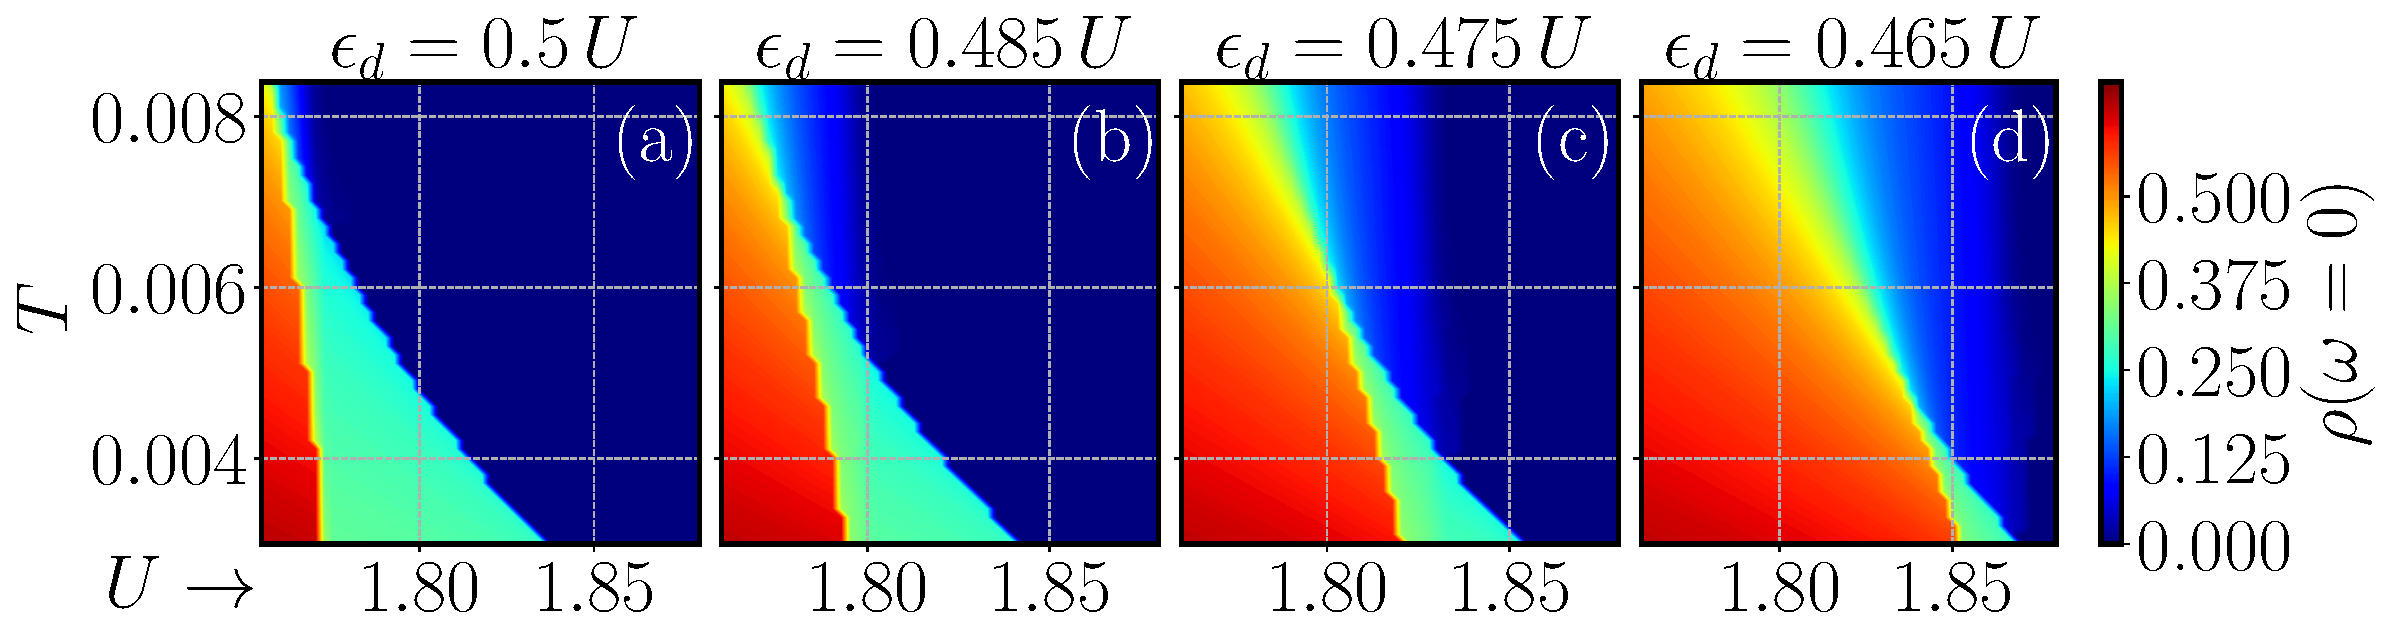
\includegraphics[width=0.7\columnwidth]{Figs/fig2-abcd-eps-converted-to.pdf}
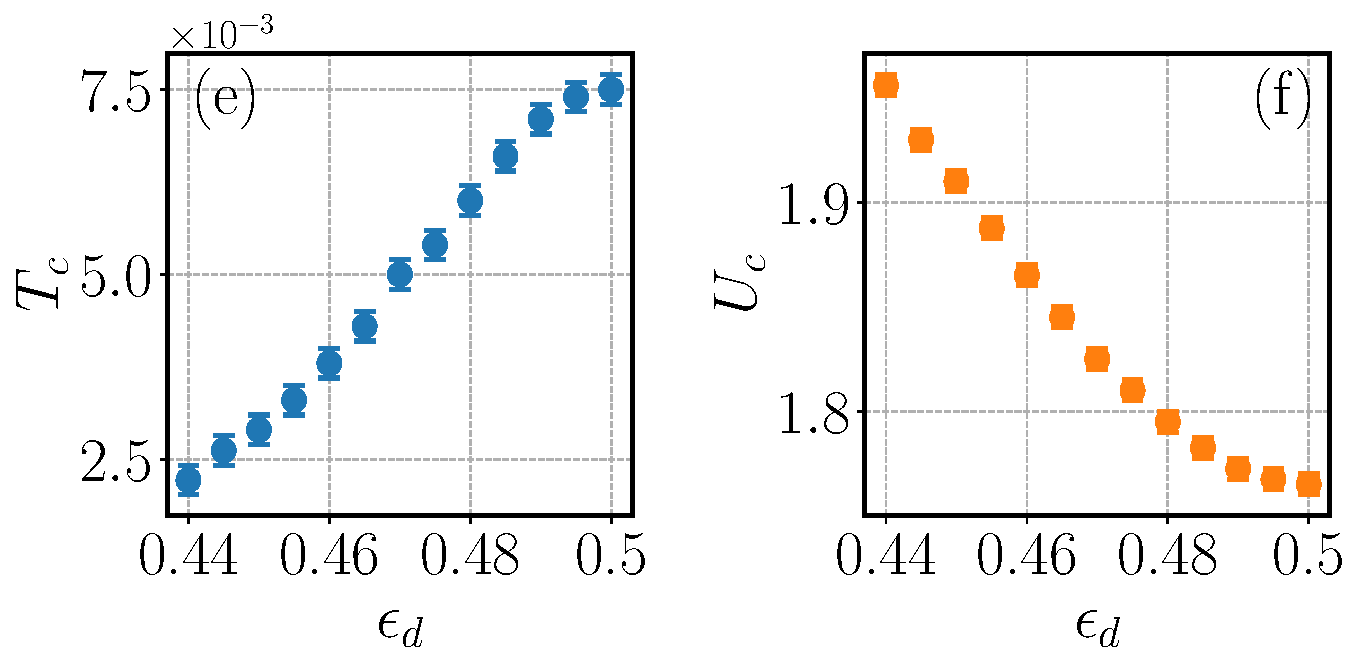
\includegraphics[width=0.42\columnwidth]{Figs/fig2-ef-eps-converted-to.pdf}
\caption{(a-d) Phase diagrams $U \times T$ as $\eps_d$ is moved away from $U/2$. (a) $\epsilon_d=0.5U$ (b) $\epsilon_d=0.485U$ (c) $\epsilon_d=0.475U$ (d) $\epsilon_d=0.465U$. (e-f) $U_c, T_c$ as functions of $\eps_d/U$. }
\label{fig:UxT-rho0}
\end{figure}

Figure \ref{fig:T0002-butterfly} shows $U \times \eps_d$ phase diagrams for the fixed temperature $T = 0.002$, where $\Delta \rho(0) = \rho_{\text{metal}}(0) - \rho_{\text{insul}}(0)$, $n = (n_{\text{metal}} + n_{\text{insul}})/2$, $\Delta n = n_{\text{metal}} - n_{\text{insul}}$. The ``smile pattern'' of Figures \ref{fig:T0002-butterfly}(a,b,d) characterize the coexistence region.

\begin{figure}[H]
\centering
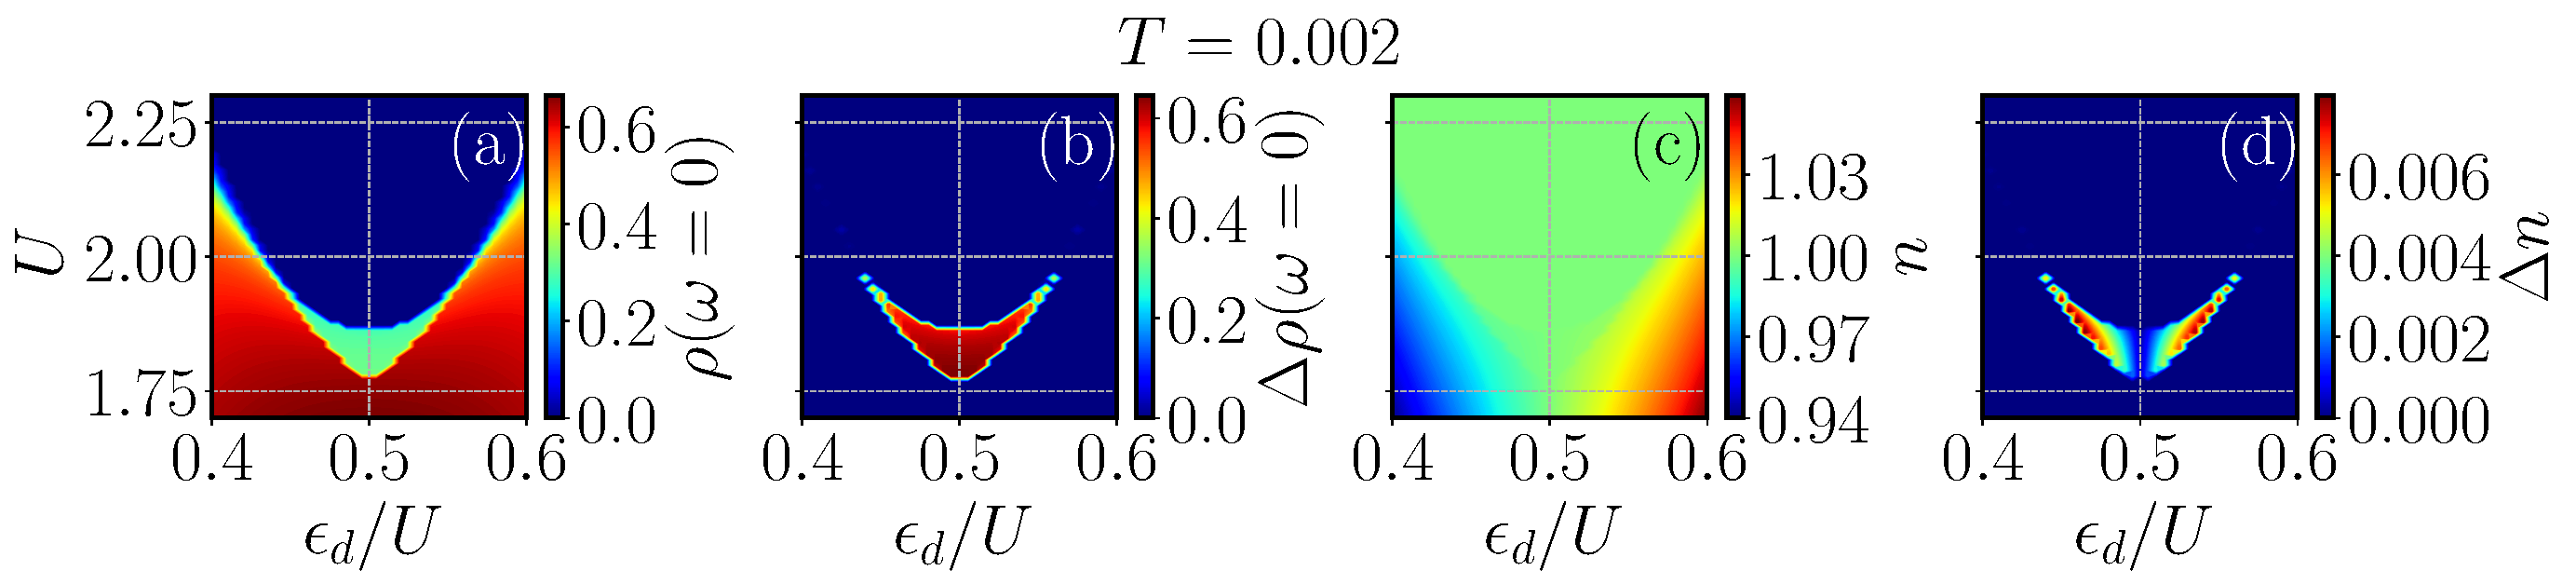
\includegraphics[width=\columnwidth]{Figs/fig4-abcd-eps-converted-to.pdf}
\caption{Phase diagrams $U \times \epsilon_d$ for $T=0.002$. (a,b) avg. $(\text{M}+\text{I})/2$ and diff. $(\text{M}-\text{I})$ for $\rho(\omega=0)$. (c,d) avg. and diff. for the filling $n$. }
\label{fig:T0002-butterfly}
\end{figure}




\section{\ALERT{Bilayer graphene}} \label{sec:tbg}


\subsection{TBG Geometry} \label{sec:tbg_geom}

The TBG system can be characterized by a rotation angle $\theta$ from the initial AB stacking stable setting. The two slightly misaligned layers then from an interference Moiré pattern, which can be commensurate (form a superlattice) or not. In the commensurate case, one can define primitive lattice vectors $\vb{L}_1$, $\vb{L}_2$ as the least common multiple of the unit vectors of two layers. Figure \ref{fig:latvec} shows an example of this.

\begin{figure}[H]
\centering
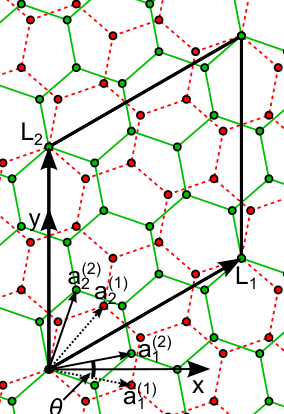
\includegraphics[width=0.4\textwidth]{fig/tbg/latvec.png}
\caption{Commensurate angle case and lattice vectors $\vb{L}_1$, $\vb{L}_2$. Figure taken from \cite{koshino2012}.}
\label{fig:latvec}
\end{figure}

As drawn in Figure \ref{fig:latvec}, we have
\begin{align}
\label{eq:scalarprods1}
\vb{a}_1^{(1)} \vdot \vb{a}_2^{(1)} &= a^2 \cos(60^\circ) = a^2/2; \\
\label{eq:scalarprods2}
\vb{a}_1^{(1)} \vdot \vb{a}_1^{(2)} &= a^2 \cos\theta; \\
\label{eq:scalarprods3}
\vb{a}_1^{(1)} \vdot \vb{a}_2^{(2)} &= a^2 \cos(60^\circ + \theta); \\
\label{eq:scalarprods4}
\vb{a}_1^{(2)} \vdot \vb{a}_2^{(1)} &= a^2 \cos(60^\circ - \theta).
\end{align}

The superlattice vectors $\vb{L}_1$, $\vb{L}_2$ are related by a $60^\circ$ rotation. In general, because $\vb{L}_1$ is a point that belongs to the lattices of both layers, it is written by integers $m,n,m',n'$ as
\begin{equation} \label{eq:L1}
\vb{L}_1 = m\vb{a}_1^{(1)} + n\vb{a}_2^{(1)} = m'\vb{a}_1^{(2)} + n'\vb{a}_2^{(2)}.
\end{equation}

Because there is an appropriate choice of lattice vectors $\vb{a}_1^{(1)}, \vb{a}_2^{(1)}, \vb{a}_1^{(2)}, \vb{a}_2^{(2)}$ (satisfying equations \ref{eq:scalarprods1} to \ref{eq:scalarprods4}) such that the indices $(m',n')$ can be made equal to $(n,m)$ \cite{koshino2012}, then by taking the scalar products of equation \ref{eq:L1} with $\vb{a}_1^{(1)}$ and $\vb{a}_1^{(2)}$, we get
\begin{equation} \label{eq:mn-system}
\begin{cases}
\; mn + n^2/2 = n^2 \cos\theta + mn \qty(\frac{\cos\theta}{2}
- \frac{\sqrt{3} \sin\theta}{2}); \\
\; m^2/2 + mn = m^2 \cos\theta + mn \qty(\frac{\cos\theta}{2}
+ \frac{\sqrt{3} \sin\theta}{2}).
\end{cases}
\end{equation}

Summing the two equations above gives us
\begin{equation} \label{eq:costheta}
\cos\theta = \frac{1}{2} \cdot \frac{m^2 + n^2 + 4mn}{m^2 + n^2 + mn}.
\end{equation}


By taking the norm of $\vb{L}_1$ from equation \ref{eq:L1} and using the angle relation in equation \ref{eq:costheta}, we find that the superlattice constant $L = \abs{\vb{L}_1} = \abs{\vb{L}_2}$ is given by
\begin{equation} \label{eq:}
L = a\sqrt{m^2 + n^2 + mn} = \frac{\abs{m-n}}{2 \sin(\theta/2)} \, a.
\end{equation}

The area of an unit cell of the superlattice is $A = \frac{\sqrt{3}}{2} L^2 = (m^2 + n^2 + mn) \, A_1$, where $A_1 = \frac{\sqrt{3}}{2} \, a^2$ is the area of unit cell of monolayer graphene. If we now consider the area of the Brillouin Zone (BZ), we get
\begin{equation} \label{eq:bz-volume}
\Omega = \frac{\Omega_1}{m^2 + n^2 + mn},
\end{equation}
where $\Omega_1 = (2\pi)^2/A$ is the BZ area of the monolayer and $\Omega$ is the area of the moiré mini BZ.

As an example, for $(m,n) = (1,2)$ we have $\theta = 21.8^\circ$ and $m^2 + n^2 + mn = 7$, therefore the monolayer BZ fits 7 mini BZ's in its area, as we see in Figure \ref{fig:bzminibz}.
\begin{figure}[H]
\centering
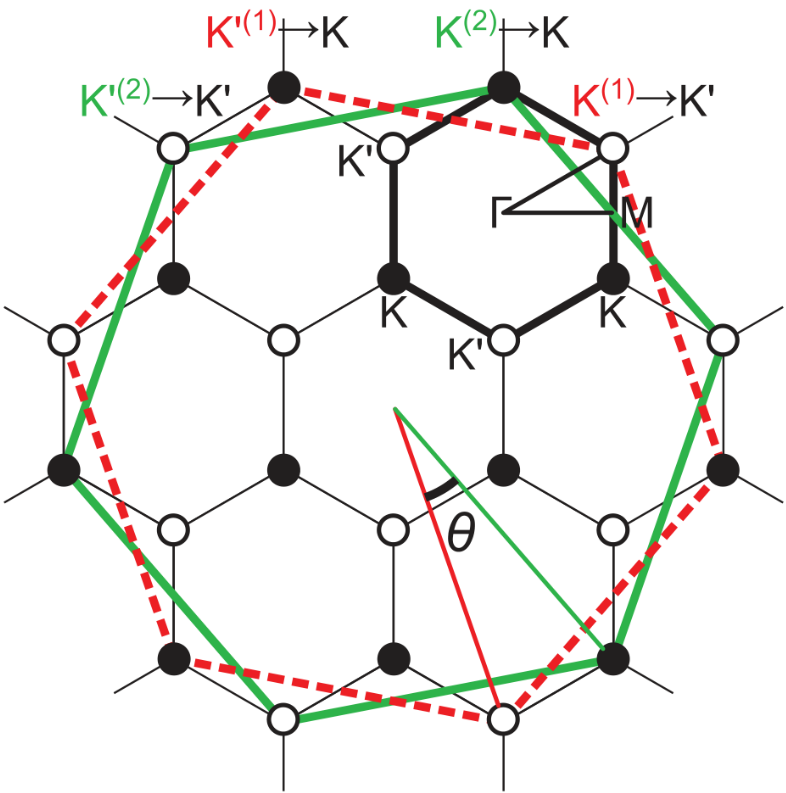
\includegraphics[width=0.4\linewidth]{fig/tbg/bzminibz.png}
\caption{Monolayers (red and green) and mini BZ's with $(m,n) = (1,2)$ and $\theta = 21.8^\circ$. Figure taken from \cite{koshino2012}.}
\label{fig:bzminibz}
\end{figure}



\chapter{Evaluation of the Institutional Support received during the period} \label{chp:apoioInst}
%\chapter{Description and evaluation of the Institutional Support received during the period} \label{chp:apoioInst}

During the period covered by this report, the student used the Research Overhead to acquire the Acer Nitro 5 AN515-58-58W3 laptop, which was extensively used for the heavy DMFT calculations in Section \ref{sec:results}.



\chapter{Participation in scientific events} \label{chp:particEvento}

The student attended the following scientific events/courses:

\begin{itemize}
\item Listener at \href{https://www.ictp-saifr.org/qm2023/}{Workshop on Strong Electron Correlations in Quantum Materials: Inhomogeneities, Frustration, and Topology}.
\item Listener at \href{https://www.ictp-saifr.org/apsmarch23/}{APS/ICTP-SAIFR Satellite March Meeting}.
\item Member of Luis Gregório G. V. Dias da Silva's research group Journal Club.
\item Attended the \href{https://american-chemical-society.zoom.us/webinar/register/WN_FISEv0_ySkK2jPVB0nbsRw#/registration}{2023 ACS Communication and Scientific Writing Course}.
\item Presented \ALERT{a poster of his DMFT results} at \href{https://www1.fisica.org.br/~eosbf/2024/index.php/en/}{2024 Autumn Meeting of the Brazilian Physical Society}.
\end{itemize}


\chapter{\ALERT{Conclusions and Future Activities}} \label{chp:conclusions}

In Section \ref{sec:hubbard} we established a fully working DMFT algorithm and were able to explore the phase diagrams for the Metal-Insulator transition. In Figure \ref{fig:UxT-rho0} we could reproduce an already known result \cite{georges1996}, but we also investigated the asymmetric case, which is a little more obscure in the literature. In particular, in Figure \ref{fig:T0002-butterfly} we were able to identify the growth of the coexistence region as $\eps_d$ approaches the symmetric case $U/2$ and the ``smile'' pattern in the $U \times \eps_d$ phase diagram in Figure \ref{fig:T0002-butterfly}. With respect to our DMFT code, we expect to improve and extend the algorithm to multi-orbital systems in order to study the TBG.

In Section \ref{sec:tbg} we shared a little of what we studied about the TBG, but there is a lot more to understand. Firstly, we hope to fully understand the structure and implications of the BM model \cite{macdonald2011}. After that, we are going to focus on studying all the symmetries and topological issues in the topological heavy fermion model \cite{topoheavyfermion2022}. This will enable us to make progress on the practical DMFT implementation of TBG system.

%%-----
%% Referências bibliográficas
%%-----
\addcontentsline{toc}{chapter}{\bibname}
%\bibliographystyle{abntex2-num}
\bibliography{bibliografia}
\bibliographystyle{ieeetr}


%%-----
%% Fim do documento
%%-----

\end{document}
